\chapter{Introduction}

\section{Context}

Design permeates engineering.
According to Ashby \citep{ashbyMaterialsSelectionMechanical1999}, the main features of mechanical design are function, material, shape, and process.
There is a profound interplay between all these facets of design when developing a mechanical component.
Accordingly, the component must meet functional criteria in terms of its thermomechanical behavior.
Additional specifications of its electric, magnetic, or mass transfer characteristics may also be prescribed.
The aptitude of a component to satisfy these demands is determined by the material or materials from which it is made, as well as its shape.
Some materials, however, cannot be manufactured into a particular shape or by using a specific manufacturing process.
Weight, cost, and environmental impact reduction can all be included as goals, and their achievement is closely related to the material and method selected.

An even more intimate relationship between the final performance of the mechanical component and the process selected for its manufacturing may be uncovered by taking into account the hierachical structure of engineering materials.
Olson \citep{olsonDesigningNewMaterial2000} emphasizes the cause/effect relationship between the process, the material's structure at multiple scales ranging from the nanoscale to the macroscale, the material's properties, and its final performance.
The reverse goals/means perspective can also be adopted where a given performance requirement drives the search for a material with a particular set of properties.
These in turn may only be realised if the appropriate multi-scale structure is obtained through a suitable process.
Ashby \citep{ashbyMaterialsSelectionMechanical1999} highlights that first-order differences between the properties of materials, e.g., polymers and metals, are due to the mass of the atoms, the nature of the inter-atomic forces and the geometry of the atomic packing.
The magnitude of the effect due to the microstructure on the properties of a material is generally an order of magnitude less than that of bonding and structure.

"Integrated Computational Materials Engineering" (ICME) is a systematic approach proposed by Horst and Wang \citep{horstemeyerCradletograveSimulationbasedDesign2003} that includes the process-structure-property-performance relationships within a computational framework.
Its goal is the simultaneous design of a component, the materials that it is composed of and the manufacturing process employed to produce it, taking into account the material's structure at different scales.
To realize this vision, suitable models and numerical tools for simulating manufacturing processes and component life at a given time and length scale must be available.
Experimental methods to probe the model's validity and acquire the corresponding material parameters are also crucial.
To accurately capture the behavior of the material, the correct boundary conditions, initial conditions, and material parameters must be established at each scale and time-frame.
An adequate way to transfer information between the different scales must also be devised.

Taking into account the hierarchical nature of a material's structure, appropriate models must be set up at the structural (meters, centimeters), macro (millimeters), meso (hundreds to tenths of micrometers), micro (micrometers), and atomic/nanoscale (angstrom).
Directly relevant to this work are both the structural and the macroscale scales.
Concerning the first, solutions from FEM are used to model the thermomechanical behavior both during manufacturing and the service life of a component or machine, with full-scale experiments being needed to gauge the accuracy of the predictions.
To achieve such a description, an appropriate constitutive/rheological model must be devised at the macroscale.
Its validation is performed through its use in suitable FEM simulations and comparison with simple mechanical experiments, e.g., uniaxial or torsion experiments.
An even more faithful description of a polymer blend, for example, may be achieved by retaining the appropriate continuum constitutive models and including an accurate mesoscale representation employing, for example, computational homegenization.
However, this is outside the scope of the present work.

\section{Motivation}

The current work focuses on two aspects of the paradigm mentioned above: the use of FEM to predict the structural response of a component under multi-physics constraints, particularly those involving thermomechanical phenomena, and the macroscale constitutive description of semi-crystalline polymers.
As such, the following sections provide two brief introductions to each topic.

 \subsection[Multi-physics simulations]{Multi-physics simulations \except{}{\protect\footnote{Adapted from \cite{vila-chaNumericalAssessmentPartitioned2023a}.}}}\label{sec:multi_physics_sims}

It is generally understood that thermomechanics is crucial in the description of many  engineering applications and a highly sought-after feature in computational models.
Thermomechanical effects play a central role in mainstream and heavy-duty applications such as rocket nozzles \citep{kuhl2002ThermomechanicalAnalysisOptimization,danowski_monolithic_2013}, disk brakes and clutches \citep{yevtushenko2015NumericalAnalysisThermal}, heat-assisted incremental sheet forming \citep{liu2018HeatassistedIncrementalSheet} and thermal stresses due to machining \citep{elsheikh2021ComprehensiveReviewResidual}, to name a few examples.
There is a profound interplay between the mechanical and the thermal field:
\begin{itemize}
  \item the thermal field influences the mechanical field through additional thermal stresses and potentially temperature-dependent material properties;
  \item  the mechanical field affects the thermal field through coupling terms, which can be interpreted as heat sources (dissipation and thermomechanical structure heating), as well as through geometric coupling due to the deformation of the domain, which affects boundary conditions and the heat conduction law.
\end{itemize}

More sophisticated applications, such as the sintering process inspired by a Hybrid FAST process described in \cite{rotheAnalyticalNumericalTreatment2014}, also exist, where a direct current and an external heat source using convection are used to control the temperature in the die/punch/powder system.
As a result, an appropriate description of the electric, thermal, and mechanical fields, as well as their interaction, must be taken into account.

Returning to the thermomechanical problem, its thermodynamically consistent formulation is necessary for the development of an appropriate solver.
Having achieved an appropriate formulation of the problem, the Finite Element Method can be used to solve it.
After spatial and temporal discretization, the thermomechanical problem is reduced to a system of coupled nonlinear algebraic equations on the mechanical variables (displacement) and thermal variables (temperatures).
Generally speaking, the strategies typically employed to solve this problem can be classified into monolithic and partitioned approaches.
The latter can be further divided into explicit (loosely or weakly coupled) and implicit (strongly coupled) schemes, depending on the type of coupling enforcement.
When comparing them, one should keep in mind that the most desirable properties of an algorithm for solving coupled problems are unconditional stability, high accuracy, ease of implementation, low memory requirements, high computational efficiency, and the potential for software reuse \citep{fellipa_partitioned_1988}.
Although a significant fraction of scientific research on solution techniques for coupled multi-physics problems has not originated from the thermomechanics community but rather from the Fluid-Structure Interaction field, the following sections present a review of these concepts linked with thermomechanics literature.
Conversely, the observations and results provided in this work in the context of thermomechanics may be generalized to other multi-physical phenomena.

\subsubsection{Monolithic schemes}
\label{sec:monolithic-schemes}

Monolithic algorithms solve the nonlinear multi-physics system of equations simultaneously, fulfilling the coupling conditions exactly.
Together with implicit time-integration techniques, monolithic schemes can provide unconditional stability and are typically associated with good robustness.
These methods are often typified by the direct application of Newton's method to the coupled equations, requiring the computation of the cross-derivative blocks between fields.
To solve the potentially large system of equations arising from the application of Newton's method, iterative methods are preferable to direct methods, partly due to memory footprint considerations.
Newton-Krylov methods with the generalized minimal residual method (GMRES) or the biconjugate gradient stabilized method (BiCGStab) as Krylov subspace solvers are among the most widely used in multi-physics problems  \citep{hron_monolithic_2006}.
The effective solution of a large system of equations, including any potential nonlinearities, is particularly difficult for monolithic algorithms \citep{danowski_monolithic_2013}, as the algebraic properties of different blocks can be very distinct.
In fact, a good preconditioning strategy is a key component of effective solvers for large-scale multi-physics problems and this has been the main development topic of monolithic schemes in the last decade \citep{tezduyar2006space, lin_parallel_2010, gee_truly_2011, danowski_monolithic_2013, verdugo_unified_2016, mayr_hybrid_2020}.
In short, the great appeal of monolithic schemes is the robustness and stability of the solution method, which comes at the expense of poor flexibility as well as extensive development and maintenance costs.

Monolithic schemes have been successfully  used in the literature to tackle thermomechanical problems considering a variety of constitutive behaviors.
Carter and Booker \citep{carter_finite_1989} consider thermoelastic materials, Gawin and Schrefler \citep{gawinThermoHydroMechanical1996} deal with thermo-hydro-mechanical problems in partially saturated porous materials, while Ibrahimbegovic and Chorfi \citep{ibrahimbegovic_covariant_2002} present a thermoplasticity covariant formulation, including large viscoplastic strains, strain localization, and cyclic loading cases.
Danowski \citep{danowski_computational_2014} deals with various temperature-dependent, isotropic, elastic, and elastoplastic material models for small and finite strains, incorporating the effect of high temperatures predominating in rocket nozzles.
Both Netz \citep{netz_high-order_2013} and Rothe and coworkers \citep{rothe_monolithic_2015} present monolithic approaches, based on the multilevel Newton method, for the solution of the thermomechanical problem involving thermovisco-plastic materials.
More recently, Felder and coworkers \citep{felder_thermomechanically_2021} proposed a finite strain thermomechanically coupled two-surface damage-plasticity theory.
The authors obtain the solution for the three coupled fields, displacement, nonlocal damage variable, and temperature, employing an implicit and monolithic solution scheme.
Relevant application of monolithic solution schemes to thermomechanical contact interaction can be found in \citet{zavarise1992RealContactMechanisms,wriggers1993ThermomechanicalContactRigorous,oancea1997FiniteElementFormulation,hueber2009ThermomechanicalContactProblems,dittmann2014IsogeometricAnalysisThermomechanical,seitz2018ComputationalApproachThermoelastoplastic}.

\subsubsection{Partitioned schemes}
\label{sec:partitioned-schemes}

The earliest contributions regarding the partitioned treatment of coupled systems emerged in the mid-1970s, involving structure-structure interactions and fluid-structure interactions (see, e.g., \cite{belytschko_mesh_1976}, \cite{park_stabilization_1977}, \cite{belytschko_stability_1978}, \cite{hughes_implicit-explicit_1978} and \cite{belytschko_mixed_1979}).
There are usually many ways of partitioning a complex system into subsystems or fields.
Felippa and Park \citep{felippa_staggered_1980} provide a very pragmatic and helpful criterion for selecting the fields to be considered.
According to their definition, a field is characterized by computational considerations.
It is a segment of the overall problem for which a separable software module is either available or readily prepared if the interaction terms are suppressed.
As such, a partitioned approach to the solution of multi-physics problems employs analyzers specific to each field separately integrated in time.
The coupling between the fields is achieved through proper communication between the individual components using prediction, substitution, and synchronization techniques.
Although this renders a flexible and easy-to-implement solution scheme, it suffers from some numerical issues, as discussed shortly.

As previously stated, partitioned schemes can be either explicit or implicit.
In explicit schemes, the solution is found by solving each field sequentially with a one-directional data transfer, using a suitable problem split.
In one exemplary time step, an explicit coupling algorithm solves the mechanical problem first, then sends relevant data to the thermal solver, and finally solves the thermal problem without providing feedback on the thermal solution to the mechanical solver.
It has been used in the context of thermoelasticity \citep{argyris_natural_1981, armero_new_1992, johansson_thermoelastic_1993, miehe_entropic_1995, miehe_theory_1995, holzapfel_entropy_1996}, thermoplasticity \citep{armero_new_1992, armero_priori_1993, simo_associative_1992, wriggers_coupled_1992, agelet_de_saracibar_numerical_1998, agelet_de_saracibar_formulation_1999,lee2015NumericalModelingAnalysis}, thermoviscoplasticity \citep{adam_numerical_2002,adam_thermomechanical_2005,miehe2011CoupledThermoviscoplasticityGlassy} and contact \citep{wriggers1994ContactConstraintsCoupled,agelet_de_saracibar_numerical_1998,xing_three_2002,bergman2004FiniteElementModel}.
The isothermic and adiabatic splits are the most common operator splits in thermomechanical problems.
The isothermal split is arguably the most straightforward and natural approach, as noted in \cite{argyris_natural_1981}, one of the earliest contributions on the topic.
This scheme seeks to solve the thermomechanical problem by first solving the mechanical problem at a constant temperature and then solving a purely thermal phase at a fixed configuration---newly updated.
As an alternative, Armero and Simo \citep{armero_new_1992} proposed the adiabatic split, which consists of a mechanical phase at constant entropy, followed by purely thermal conduction at fixed configuration.
In terms of implementation complexity, the adiabatic split is comparable to the isothermal split and is unconditionally stable, a remarkable advantage in comparison with the conditionally stable isothermal split.
It is, however, more challenging to extend to other material models as it requires the modification and creation of specific algorithmic components at the constitutive level which might not be readily available.

There are several techniques to improve the stability and accuracy characteristics of explicit partitioned approaches, e.g., algebraic augmentation \citep{park_stabilization_1977, park_stabilization_1983}, double-pass approach \citep{armero_new_1992, piperno_explicitimplicit_1997, farhat_provably_2006, farhat_robust_2010}, prediction techniques \citep{piperno_explicitimplicit_1997, piperno_partitioned_2001, michler_efficient_2005, farhat_provably_2006}, and subcycling \citep{piperno_partitioned_1995, farhat_high_1997, piperno_explicitimplicit_1997}.
Irrespective of the theoretical temporal convergence order of the partitioned explicit scheme, the fully coupled discretized equations of the problem will never be exactly satisfied at each time instant.
There is a lag between the solution of the different fields, e.g., the mechanical and thermal fields, in a thermomechanical problem, which can be interpreted as an additional discretization error \citep{michler_efficient_2005}.
The convergence conditions of partitioned solution procedures are also discussed by Turska and Schrefler \citep{turskaConvergenceConditionsPartitioned1993a} in the context of consolidation problems.

In implicit schemes, inter-field iterations are performed until a given tolerance for the different field's unknowns is reached---irrespective of the type of operator split employed.
It converges to the solution of the monolithic scheme and thus can satisfy the discrete version of the coupled problem exactly.
Regardless of the eventual conditional stability of the corresponding explicit scheme, the implicit alternative can be unconditionally stable---it has the same temporal stability properties as the monolithic scheme---but the convergence of the inter-field iterations is not guaranteed or may take an excessive number of iterations.
This embodies a significant limitation and places a severe restriction on the use of these strategies.
Nonetheless, several acceleration techniques are available in the literature to speed up convergence.
Most of these are developed in the context of Fluid-Structure Interaction and their application to thermomechanical problems is not widespread.

There are a few contributions regarding the use of implicit partitioned schemes in the context of thermomechanics.
Erbts and Düster \citep{erbts_accelerated_2012} solve problems involving thermoelasticity at finite strains, Netz \citep{netz_high-order_2013} explores thermoviscoelastic problems, and Da\-now\-ski \citep{danowski_computational_2014} presents results on thermoelasticity and thermoelastoplasticity.
Including more than two fields, Erbts and coworkers \citep{erbts_partitioned_2015} tackle electro-thermomechanical problems, as do Wendt and coworkers \citep{wendt_partitioned_2015}, which also consider radiative heat transfer.
Successful applications to thermomechanical problems involving contact have been reported in \citet{johansson_thermoelastic_1993,rieger2004AdaptiveMethodsThermomechanical,temizer2011ThermomechanicalContactHomogenization,kruger2020PorousductileFractureThermoelastoplastic}, to name a few.

Regarding computational efficiency, according to Michler \citep{michler_efficient_2005}, solving a fluid-structure interaction problem to the same accuracy using an explicit scheme is less efficient than employing an implicit approach.
For the same total number of iterations, the difference in the accuracy reached ranges from one to three orders of magnitude---although the implicit coupling is more expensive for the same number of iterations, naturally.
These findings contradict a claim made in \cite{felippa_partitioned_2001}, which is not supported by any numerical results.
In the numerical examples presented in \cite{danowski_computational_2014}, the monolithic solver is, in most cases, faster than an implicit scheme employing Aitken relaxation for problems in thermomechanics.
The differences range from 120\% to 140\% in favor of the monolithic scheme.
Supporting evidence for these conclusions can also be found in \cite{novascone_evaluation_2015}.
The authors report  CPU time ratios between the implicit partitioned and monolithic approaches, ranging from 0.635 to 3.75 on the coupling magnitude.
This evidence suggests that implicit schemes can deliver competitive simulation times with the same accuracy as the monolithic if more sophisticated coupling techniques are used to accelerate the convergence and improve the robustness of the inter-field iterations, with the added benefit of more straightforward implementation and extension.

Lastly, it is important to recall the recommendations given in \cite{felippa_partitioned_2001} regarding the choice between partitioned and monolithic approaches.
According to the authors, the circumstances that favor the partitioned approach for tackling a coupled problem are a research environment with few delivery constraints, access to existing software, localized interaction effects, and widespread spatial/temporal component characteristics.
The opposite circumstances, involving a commercial environment, a rigid deliverable timetable, massive software development resources, global interaction effects, and comparable length and time scales, favor a monolithic approach.
Therefore, one can readily see a number of applications where partitioned strategies fit very well, involving small development times and preservation of pre-existing technology.

\subsection{Semi-crystalline polymers}

The majority of polymeric materials are made up of extremely long molecule chains with side groups composed of different elements, such as O, F, or Cl, or organic groups, like methyl, ethyl, or phenyl groups.
These macromolecules comprise repeat units, which are smaller structural elements replicated along the chain \citep{callister2014materials}.
In turn, the polymer structure can range from a completely amorphous polymer, where the macromolecules are arranged randomly, to a highly crystalline polymer, where most polymer chains are tightly packed into a crystalline structure.
In between, one finds semi-crystalline polymers where crystalline and amorphous zones coexist in a variety of structural arrangements \citep{wardIntroductionMechanicalProperties2004}.

\subsubsection{Properties and applications}

According to a market study by Precedence Research \citep{precedenceresearchPolymersMarketProduct2022}, the polymer market size in 2021 was 713 billion dollars, and it is projected to reach 1078.5 billion by 2030.
By type, the thermoplastics segment accounted for 43\% market share in 2021.
Most semi-crystalline polymers are designated as thermoplastics, as they most often have linear structures and soften/harden when heated/cooled.
Thermoplastics dominate the market due to their reduced production costs, energy efficiency, ability to replace metals with considerable weight savings, and ability to be produced in extremely high volumes with high precision and cheaply.

By material, the polyethylene (PE) segment, a semi-crystalline polymer, has captured a significant market share in 2021 and is growing.
It is widely sought after for packaging items, tubing products, connections, bottles, and plastic surgery implants.
Increased consumer spending and industrial operations across various industries, including the automobile, building, and packaging, are the main drivers of this increase.
Another widely used semi-crystalline polymer is polytetrafluoroethylene (PTFE), employed in many medical and industrial device applications, in particular, in rotary shafts seals, due to its tribological characteristics, chemical inertness and temperature stability \citep{kletschkowskiEndochronicViscoplasticMaterial2002}.
Polyamides (PA) are widely used materials due to their low material cost, low density (approximately 12.5\% the weight of bronze, 14.3\% the weight of cast iron, and 50\% the weight of aluminum),  corrosion resistance, insulation qualities, and good load bearing capacity.
They are frequently used as replacement for bronze, brass, aluminum and other metals \citep{khanThermomechanicalResponseNylon2006}.
PA6 is used in conjunction with PE in polymer films for food packaging, due to its good mechanical strength and impermeability to gas \citep{zengConstitutiveModelSemicrystalline2010}.
Polyether ether ketone (PEEK) is yet another semi-crystalline polymer which finds use in a variety of structural and insulation applications \citep{raeMechanicalPropertiesPoly2007}.
Moreover, due to its excellent mechanical properties, PEEK is commonly used in seals and bearings, and more recently also in medical implants (e.g., spinal implants, screws, woven textiles) \citep{bergstromMechanicsSolidPolymers2015}, due to its biocompatibility, weight reduction, radiology advantage and 3D printing properties \citep{garcia-gonzalezMechanicalImpactBehavior2015}.
Its exceptionally high melting temperature also makes it a good candidate for extreme service conditions \citep{gsellEvolutionMicrostructureSemicrystalline1994}.
% MOre applications rtp


\subsubsection{Semi-crystalline polymer structure}

Semi-crystalline polymers have a complex and hierarchial heterogeneous morphology.
Both their microstructure and their mesostructure will depend on the processing history, as well as mechanical and thermal histories, in addition to the polymer chemistry and conformation \citep{khouryMorphologyCrystallineSynthetic1976,cangemiTwoPhaseModelMechanical2001,hoffmanAnalysisRelaxationsPolychlorotrifluoroethylene2007}.

\paragraph{Microstructure}
At the microscopic level, semi-crystalline polymers consist of at least two different phases: a crystalline phase and an amorphous phase \citep{khouryMorphologyCrystallineSynthetic1976}.
The crystalline portion of a semi-crystalline polymer is formed by the constituent chains packing parallel to one another into lamellae in an orderly fashion, as shown in Figure~\ref {fig:crystalline_phase_of_scp}.

\begin{figure}[htbp]
  \centering
	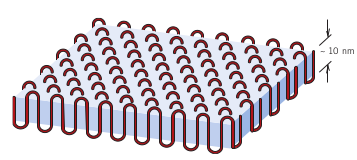
\includegraphics[width=0.6\textwidth]{figures/crystalline_phase_of_scp}
	\caption{Arrangement of polymer chains into a lamella in the crystalline phase of a semi-crystalline polymer \citep{callister2014materials}.}
\label{fig:crystalline_phase_of_scp}
\end{figure}

There are at least two types of crystal lamellae found in semi-crystalline polymers, as detailed in \cite{andersonMorphologyIsothermallyBulk1964} for polyethylene (PE), the chain-folded lamellae and extended-chain lamellae.
In the former, the molecular chains within each platelet fold back and forth on themselves, with folds occurring at the faces.
This picture is, in fact, an idealization, with reality resembling more a switchboard model, with the chains reentering through loose folds at non-adjacent sites or even forming tie-chains with neighboring lamellae \citep{gsellEvolutionMicrostructureSemicrystalline1994}.
The latter is more common at lower molecular weights, with the chains organized into lamellae in their extended conformation.
The thickness of the lamellae in semi-crystalline polymers is of the order of nanometers, e.g., \SIrange{10}{15}{\nano\meter} for PE samples \citep{argonPhysicsDeformationFracture2013a}.
% \begin{figure}[hbtp]
% 	\includegraphics{example-image-a}
% 	\caption{Schematic depictions of chain-folded and extended-chain lamellae.}
% \label{fig:types_of_crystall}
% \end{figure}

The crystalline structure depends on the particular polymer.
PE often possesses orthorhombic symmetry, where the chain direction forms an angle with the normal vector to the crystalline lamella ranging between $17^\circ$ and $40^\circ$ \citep{nikolovMicroMacroConstitutive2000}.
On the other hand, the crystal structure found in polytetrafluoroethylene (PTFE) at temperatures above \SI{19}{\celsius} is hexagonal, with individual molecules arranged in helical conformations \citep{bergstromMechanicsSolidPolymers2015}.
% See Figure~\ref{fig:crystalline_structure_PE_PTFE} for a depiction of both crystalline structures.
% \begin{figure}[hbtp]
% 	\includegraphics[width=0.9\textwidth]{example-image-a}
% 	\caption{Depiction of the crystalline structures of polyethylene (PE) and polytetrafluoroethylene (PTFE).}
% \label{fig:crystalline_structure_PE_PTFE}
% \end{figure}

The crystallinity of a semi-crystalline polymer can be specified by the degree of crystallinity.
It may range from completely amorphous to almost entirely crystalline.
Ward and Sweeney \citep{wardIntroductionMechanicalProperties2004} mention values between $90\%$ for polyethylene (PE) to about $30\%$ for oriented poly(ethylene terephthalate) (PET).
Commercially available semi-crystalline polymers range from $10\%$ to $90\%$ in the degree of crystallinity \citep{vandommelenMicromechanicalModelingElastoviscoplastic2003}.
The degree of crystallinity by weight may be determined from accurate density measurements according to
\begin{equation}
	\chi = \% \text { crystallinity }=\frac{\left(\rho_{s}-\rho_{a}\right)/\rho_{s}}{\left(\rho_{c}-\rho_{a}\right)/\rho_{c}} \times 100
\end{equation}
where $\rho_{s}$ is the density of a specimen for which the percent crystallinity is to be determined, $\rho_{a}$ is the density of the completely amorphous polymer, and $\rho_{c}$ is the density of the perfect polymer crystallite.
In addition to this method based on density, other experimental methods employed to determine the crystallinity along with the lamellar thickness of the polymer crystallites include wide (WAXS) and small (SAXS) angle X-ray scattering \citep{schrauwenIntrinsicDeformationBehavior2004, hobeikaTemperatureStrainRate2000}, differential scanning calorimetery (DSC) \citep{ayoubEffectsCrystalContent2011}, and, electron microscopy, e.g., transmission electron microscopy (TEM) \citep{bartczakEvolutionCrystallineTexture1992}.

The main parameters influencing the degree of crystallinity are the molecular structure, the molecular weight, the presence of plasticizers, and especially the thermomechanical history of the polymer \citep{khouryMorphologyCrystallineSynthetic1976, cangemiTwoPhaseModelMechanical2001}.
Because of the way polymer crystals form, polymer chains must have a linear structure; the more branches/dependent side groups, the lower the degree of crystallinity.
However, even linear polymers must have sufficient regularity to crystallize \citep{khouryMorphologyCrystallineSynthetic1976}.
A high molecular weight tends to suppress a high degree of crystallinity \citep{hoffmanAnalysisRelaxationsPolychlorotrifluoroethylene2007}, as seen when comparing high-density polyethylene (HDPE) and ultra-high weight polyethylene (UHWPE) \citep{brownInfluenceMolecularConformation2007}.
Since crystallization is a kinetic process, the crystallization rate in polymers depends on the temperature, with larger temperatures leading to lower rates \citep{callister2014materials}.
As detailed later in this chapter, the mechanical loading of a polymer may also induce changes in crystallinity, e.g., through the phenomenon of strain-induced crystallization \citep{raoStudyStraininducedCrystallization2001}.

Accordingly, the most frequent approach to achieve different degrees of crystallinity is through the control of crystallization temperatures and crystallization times, be it when crystallizing from the melt or through annealing treatments \citep{fakirovGlassTransitionTemperature2000, schrauwenIntrinsicDeformationBehavior2004}.
However, preparing samples with different degrees of crystallinity is challenging for polymers such as HDPE since its crystallization rate is very high.
It is possible to control the degree of crystallinity by taking PE samples differing in the degree of branching and introducing various amounts of defects in the main chain \citep{fakirovGlassTransitionTemperature2000}.

In what pertains to the amorphous portion of a semi-crystalline polymer, results reported by Zia and coworkers \citep{ziaRigidAmorphousFraction2008} on isotactic polypropylene (iPP) point to the existence of two different amorphous phases, a mobile amorphous phase, and a rigid amorphous phase, based on different glass transition temperatures.
The results of Jolly \citep{jollyAnalyseMicrostructurePolyamide2000} concerning polyamide 11 (PA11), which were found employing WASX at different axial deformation rates, also support the existence of a phase that is neither wholly amorphous nor wholly crystalline.
According to Mandelkern \citep{mandelkernCrystallinePolymerReminiscences2006}, the existence of a rigid amorphous phase is supported by experimental results obtained from density measurements, wide and small-angle X-ray diffraction, thermal analyses, Raman spectroscopy, small-angle neutron scattering, dielectric relaxation and nuclear magnetic resonance involving different nuclei and techniques.

The reason for the increased rigidity in this part of the amorphous phase is the presence of polymer crystallites, which hinder the molecular mobility of the amorphous phase \citep{ziaRigidAmorphousFraction2008, peacockHandbookPolyethyleneStructures2014}.
However, an increase in the degree of crystallinity will decrease the rigid amorphous fraction and the ratio between the rigid and mobile amorphous phases.
This behavior is due to reduced covalent coupling between the polymer crystals and the amorphous phase in highly crystalline preparations \citep{ziaRigidAmorphousFraction2008}.
Furthermore, the presence of the crystallites also affects the properties of the mobile amorphous fraction, which is detected by a distinct decrease in its glass transition temperature, as shown for semi-crystalline iPP by Zia and coworkers \citep{ziaRigidAmorphousFraction2008}.

\paragraph{Mesostructure}
According to the processing, thermal and mechanical history, as well as its degree of crystallinity, molecular weight, and polydispersity, a semi-crystalline polymer can display different mesoscopic structures \citep{cangemiTwoPhaseModelMechanical2001, mandelkernCrystallinePolymerReminiscences2006}.
When the polymer crystallizes from a dilute solution, the structure is often lamellar and composed of multiple layers if the solution is quiescent, and of the shish-kebab variety\footnote{The so-called shish-kebab structure consists of a long central fiber core (shish) surrounded by a lamellar crystalline structure (kebab) periodically attached along the shish.
\citep{naViscousForceDominatedTensileDeformation2006, peacockHandbookPolyethyleneStructures2014}.} if the solution is subject to high shear \citep{khouryMorphologyCrystallineSynthetic1976, callister2014materials, peacockHandbookPolyethyleneStructures2014}.
When the polymer crystallizes from the melt, the two most commonly reported types of mesoscopic structures for semi-crystalline polymers are the spherulitic structure \citep{zengConstitutiveModelSemicrystalline2010} (see Figure~\ref{subfig:spherulitic_mesostructure_scp}), obtained from quiescent crystallization and the shish-kebab structure, obtained from crystallization under shear stress \citep{peacockHandbookPolyethyleneStructures2014} (see Figure~\ref{subfig:shish_kebab_mesostructure_scp}).
\begin{figure}[hbtp]
\centering
\begin{subfigure}[c]{0.45\textwidth}
            \centering
            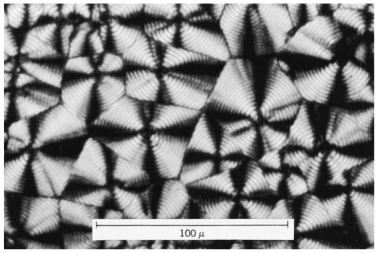
\includegraphics[width=\textwidth]{figures/spherulitic_mesostructure_scp}
            \caption{}
            \label{subfig:spherulitic_mesostructure_scp}
    \end{subfigure} \hfill
    \begin{subfigure}[c]{0.45\textwidth}
            \centering
            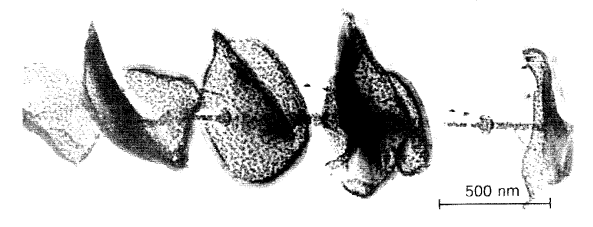
\includegraphics[width=\textwidth]{figures/shish_kebab_mesostructure_scp}
            \caption{}
            \label{subfig:shish_kebab_mesostructure_scp}
    \end{subfigure}
	\caption{Mesostructures of polyethylene. \subref{subfig:spherulitic_mesostructure_scp} Transmission photomicrograph (using cross-polarized light) of a spherulitic structure \citep{callister2014materials}. \subref{subfig:shish_kebab_mesostructure_scp} Electron micrograph of shish-kebab structure \citep{peacockHandbookPolyethyleneStructures2014}.}
\label{fig:mesostructure_scp}
\end{figure}

The spherulitic structure is composed of spherulites, an aggregate of ribbon-like chain-folded crystallites that radiate outward from a single nucleation site in the center, their diameter approximately \SI{10}{\micro\meter} and their lammela approximately 10 to \SI{20}{\nano\meter} thick for PE, and 2 to \SI{6}{\nano\meter} for polyether ether ketone (PEEK), for example.
Between them, there are amorphous regions, crossed by tie-chain molecules that act as connecting links between adjacent lamellae \citep{callister2014materials, khouryMorphologyCrystallineSynthetic1976, pouriayevaliConstitutiveDescriptionRatesensitive2013, gsellEvolutionMicrostructureSemicrystalline1994}.
The lamellae are generally twisted about their long axis \citep{patlazhanStructuralMechanicsSemicrystalline2012}.
A sheave-like structure is also possible under suitable conditions \citep{peacockHandbookPolyethyleneStructures2014}.
Mandelkern \citep{mandelkernCrystallinePolymerReminiscences2006} warns, however, that spherulites, and other types of supermolecular structures, are not universally observed in homopolymers.

Mechanical loading will also lead to changes in the mesoscopic structure of the polymer.
Regarding higher crystallinity polymers such as HDPE, it usually destroys the crystallites of the original morphology, followed by reordering to form new crystallites.
The new lamellar morphology has a lamellar thickness independent of the original lamellar thickness, solely dependent upon the temperature at which the deformation occurred.
In such morphologies, the unit cell axes are preferentially aligned in the stress direction, while the lateral planes of the lamellae lie approximately normal to the aligning force.
These newly formed crystallites are themselves subject to disruption at higher deformation levels (draw ratios of approximately 10), being replaced by a fibrillar morphology, which consists of oriented crystallites arranged hierarchically into needle-like structures of various sizes.
These macrofibrils are composed of microfibrils, in turn, made up of nanofibrils, stacks of crystallites separated by thin noncrystalline "plates," portions of which are spanned by "intercrystalline bridges" \citep{peacockHandbookPolyethyleneStructures2014}.
A nearly perfect alignment of the crystallized chains along the fiber axis and the parallel arrangement of the crystal lamellae relative to the same axis define the final fiber structure \citep{peterlinMolecularModelDrawing1971}.
Moreover, plastically deforming HDPE develops three important types of texture, resembling that of a large quasi-single crystal \citep{argonPhysicsDeformationFracture2013a}:
\begin{enumerate}
	\item crystallographic texture due to preferential orientation of crystallographic axes in the crystalline lamellae;
	\item morphological texture due to preferential orientation of the normals to the broad faces of the crystalline lamellae faces;
	\item macromolecular texture in the amorphous component, which is promoted by the alignment of molecules in the direction of maximum stretch.
\end{enumerate}

For materials such as PET, in which the crystalline and amorphous components are intermixed, the most noticeable effect may be strain-induced crystallization due to macromolecular texture, as described above \citep{wardIntroductionMechanicalProperties2004}.
More specifically, temperatures above the glass transition temperature, a linear structure, and large deformations increase the crystallinity of the material \citep{ahziModelingDeformationBehavior2003}.
The crystalline structures produced in this way are oriented, which results in an anisotropic mechanical response.
Experiments on polymer film also point to crystallization at lower strain when the strain rate is higher \citep{raoStudyStraininducedCrystallization2001}.
Most plastic products are manufactured by deforming the material at elevated temperatures to get it into the desired shape.
Examples of these operations include film blowing, fiber spinning, and injection molding.
In many of these applications, the formation of a highly oriented crystalline phase has a beneficial impact on the mechanical behavior of the material \citep{dairaniehPhenomenologicalModelFlowInduced1999, raoStudyStraininducedCrystallization2001}.
Hence, most PET articles are manufactured in this way \citep{boyceConstitutiveModelFinite2000, raoStudyStraininducedCrystallization2001, makradiTwophaseSelfconsistentModel2005}.


\section{Computational framework}

All the numerical simulations based on the Finite Element Method (FEM) are held in the in-house Fortran (IBM Mathematical Formula Translation System) program LINKS (Large Strain Implicit Nonlinear Analysis of Solids Linking Scales), a multi-scale finite element code for implicit infinitesimal and finite strain analyses of hyperelastic and elastoplastic solids, that is continuously developed by the CM2S research group (Computational Multi-Scale Modeling of Solids and Structures) at the Faculty of Engineering of University of Porto.

In the present work, the author contributes to the addition of a suitable coupling environment for the partitioned solution of coupled fields and a thermal solver based on the Finite Elements Method.
Appropriate nonlinear solvers are also added as implicit solution strategies for the coupled thermomechanical problem.

The numerical simulations concerning the solution of uniaxial traction and compression problems for validating constitutive models are run in an in-house Python program based on the implementation described in \cite{bergstromMechanicsSolidPolymers2015}.

The author contributes with two constitutive models to describe the behavior of semi-crystalline polymers.

\section{Objectives}

The main goals of this work are:
\begin{itemize}
    \item To formulate the thermomechanical problem in a thermodynamically consistent way;
    \item To provide a thorough overview of the available methods for the solution of coupled problems, in particular, the thermomechanical problem;
    \item To validate the thermomechanical solver and compare the strongly coupled partitioned strategies available in the literature;
    \item To thoroughly describe the thermomechanical behavior of semi-crystalline polymers;
    \item To review the state-of-the-art of semi-crystalline polymer constitutive modeling;
    \item To implement some of the state-of-the-art constitutive models for semi-crystalline polymers.
\end{itemize}

\section{Document structure}

The remainder of this document is structured as follows:

\paragraph{Chapter \ref{ch:thermomechanical_problem} - Thermomechanical problem}\mbox{}\\
This chapter covers the concepts required to describe how a solid responds to thermal and mechanical loads under large deformations, including the conservation laws that guarantee mechanical equilibrium and energy conservation.
Additionally, the application of thermodynamics with internal variables is discussed, along with the resulting inferences about the constitutive behavior of the solid material.
The implicit partitioned methods to solve the thermomechanical problem are also described.

\paragraph{Chapter \ref{ch:thermomechanical_behavior_semi_crystalline_polymer} - Thermomechanical behavior of semi-crystalline polymers}\mbox{}\\
This chapter attempts to outline the thermomechanical response of semi-crystalline polymers.
An account of their deformation mechanisms, experimental results of various mechanical experiments, and an appropriate discussion regarding their dependency on factors such as temperature, strain rate, or pressure is included.
This chapter also contains the results of thermal analysis techniques, such as differential scanning calorimetry.
An effort is made to provide relevant literature references where the experimental results can be found.

\paragraph{Chapter \ref{ch:modeling_semi_crystalline_polymer} - State of the art in thermomechanical semi-crystalline polymer\\ constitutive modeling}\mbox{}\\
The main goal of this chapter is to report on the semi-crystalline polymer modeling state of the art.
The departure point is infinitesimal thermoviscoelasticity.
Nonlinear generalizations are considered by specifying nonlinear laws for the elastic and viscous elements in rheological models originating from infinitesimal viscoelasticity.
These are the most commonly available models in the literature, and a detailed overview is provided in this chapter.
Following that is a description of models that distinguish between the crystalline and amorphous phases while only considering bulk crystallinity and no additional geometrical information.
Finally, multi-scale models with micro and mesostructure considerations are described.

\paragraph{Chapter \ref{ch:numerical_results} - Numerical results}\mbox{}\\
This chapter presents two sets of results concerning the thermomechanical modeling of semi-crystalline polymers.
The first is adapted from \cite{vila-chaNumericalAssessmentPartitioned2023a} and pertains to the implicit partitioned solution of a thermomechanical problem involving nonlinear elastoplastic material behavior.
The second pertains to the implementation and validation of two state-of-the-art constitutive models for semi-crystalline polymers.

\paragraph{Chapter \ref{ch:conclusions} - Conclusion and Future Works}\mbox{} \\
This chapter presents the conclusions reached in this work and discusses future research directions.
